
\section{上同调的（理想）性质}

我们并不立刻定义\trQCSheaf{}的\trCohomology，而是先讨论我们为何关心它，以及它应当具有哪些性质。

由于 $\Gamma(X,\cdot)$ 是一个\trLeftExact{}函子，若
$0\to\mathscr{F}\to\mathscr{G}\to\mathscr{H}\to 0$ 是概形 $X$ 上诸\trQCSheaf{}的一个\trShortExactSequence，则
\[
0\longrightarrow \mathscr{F}(X)\longrightarrow \mathscr{G}(X)\longrightarrow \mathscr{H}(X)
\]
是正合的。我们梦想这个序列能向右延续下去，给出一个\trLongExactSequence。更明确地说：应当存在一些协变函子
$\mathrm{H}^i$（$i\ge 0$），把 $X$ 上的\trQCSheaf{}送到\trGroup，使得 $\mathrm{H}^0$ 就是\trGlobalSections{}函子
$\Gamma$，并且有「上同调中的\trLongExactSequence」。
\begin{equation*}\tag{18.1.0.1}\label{eq:cohomology-long-exact-seq}
\begin{gathered}
0\longrightarrow \mathrm{H}^0(X,\mathscr{F})\longrightarrow \mathrm{H}^0(X,\mathscr{G})\longrightarrow \mathrm{H}^0(X,\mathscr{H})\\[10pt]
\longrightarrow \mathrm{H}^1(X,\mathscr{F})\longrightarrow \mathrm{H}^1(X,\mathscr{G})\longrightarrow \mathrm{H}^1(X,\mathscr{H})\longrightarrow\cdots
\end{gathered}
\end{equation*}

（一般地，每当我们见到一个\trLeftExact{}或\trRightExact{}的函子，都应当盼望这件事；而在好的情形里，我们的梦想将会成真。这背后的机关通常涉及\emph{\trDerivedFunctor}（derived functor），我们将在第 23 章讨论。）

在显式定义\trQCSheaf{}的各\trCohomology{}群之前，我们先描述它们的重要性质；这些性质在某些方面甚至比形式定义还要重要。加了框的性质才是重要的。

设 $X$ 是一个\emph{分离且拟紧}的 $A$-\trScheme。对 $X$ 上每个\trQCSheaf{} $\mathscr{F}$，我们都将定义 $A$-\trModule{}
$\mathrm{H}^i(X,\mathscr{F})$。特别地，若 $A=k$，它们就是 $k$-\trVectorSpace；此时我们定义
$h^i(X,\mathscr{F})=\dim_k\mathrm{H}^i(X,\mathscr{F})$（在左边，$k$ 被隐去不写）。

\textbf{(i)}\quad 每个 \fbox{$\mathrm{H}^i$ 都是从 $\mathit{QCoh}_X$ 到 $\mathit{Mod}_A$ 的协变函子}。

\textbf{(ii)}\quad 函子 $\mathrm{H}^0$ 被等同于函子 $\Gamma$：\fbox{$\mathrm{H}^0(X,\mathscr{F})=\Gamma(X,\mathscr{F})$，}而且 \textbf{(i)} 的协变性在 $i=0$ 时不过是 $\Gamma$ 的寻常协变性（$\mathscr{F}\to\mathscr{G}$ 诱导
$\Gamma(X,\mathscr{F})\to\Gamma(X,\mathscr{G})$）。

\textbf{(iii)}\quad 若 $0\to\mathscr{F}\to\mathscr{G}\to\mathscr{H}\to 0$ 是 $X$ 上诸\trQCSheaf{}的一个\trShortExactSequence，则我们有一条 \fbox{\trLongExactSequence}（\eqref{eq:cohomology-long-exact-seq}）。映射
$\mathrm{H}^i(X,\mathscr{F})\to\mathrm{H}^i(X,\mathscr{G})$ 来自协变性，
$\mathrm{H}^i(X,\mathscr{G})\to\mathrm{H}^i(X,\mathscr{H})$ 亦然；至于\emph{\trConnectingHomomorphism}（connecting homomorphism）
$\mathrm{H}^i(X,\mathscr{H})\to\mathrm{H}^{i+1}(X,\mathscr{F})$，则尚有待定义。

\textbf{(iv)}\quad 若 $\pi\colon X\to Y$ 是拟紧分离 $A$-\trScheme{}之间的任意一个\trMorphism，而 $\mathscr{F}$ 是 $X$ 上的一个\trQCSheaf，则存在自然的\trMorphism{}
\fbox{$\mathrm{H}^i(Y,\pi_*\mathscr{F})\to\mathrm{H}^i(X,\mathscr{F})$}，它是
$\Gamma(Y,\pi_*\mathscr{F})\to\Gamma(X,\mathscr{F})$ 的扩张。（注意：由关于拟紧与分离态射的\trCancellationTheorem{}~11.1.1——在该定理的陈述中取 $Z=\Spec A$——$\pi$ 确实既拟紧又分离，于是由\mbox{练习~14.4.C}，$\pi_*\mathscr{F}$ 确实是\trQCSheaf。）我们日后会看到，这是一个更大故事——\emph{\trLeray\trSpectralSequence}（\mbox{定理~23.4.5}）——的一部分。若 $\mathscr{G}$ 是 $Y$ 上的一个\trQCSheaf，则令 $\mathscr{F}:=\pi^*\mathscr{G}$，并利用伴随映射
$\mathscr{G}\to\pi_*\pi^*\mathscr{G}$ 与协变性（性质 (i)），便得到一个自然的\textbf{\trPullback{}映射}（pullback map）
$\mathrm{H}^i(Y,\mathscr{G})\to\mathrm{H}^i(X,\pi^*\mathscr{G})$（经由
$\mathrm{H}^i(Y,\mathscr{G})\to\mathrm{H}^i(Y,\pi_*\pi^*\mathscr{G})\to\mathrm{H}^i(X,\pi^*\mathscr{G})$），它是
$\Gamma(Y,\mathscr{G})\to\Gamma(X,\pi^*\mathscr{G})$ 的扩张。如此一来，$\mathrm{H}^i$ 便是「在空间上的\trContravariantFunctor」。

\textbf{(v)}\quad 若 $\pi\colon X\to Y$ 是一个\trAffine\trMorphism，而 $\mathscr{F}$ 是 $X$ 上的一个\trQCSheaf，则 \textbf{(iv)} 中的自然映射是一个\trIsomorphism：\fbox{$\mathrm{H}^i(Y,\pi_*\mathscr{F})\overset{\sim}{\longrightarrow}\mathrm{H}^i(X,\mathscr{F})$.}当 $\pi$ 是\trClosedEmbedding{}而 $Y=\mathbb{P}^N_A$ 时，这个\trIsomorphism{}把任意\trProjective{} $A$-\trScheme{}上的计算转译为 $\mathbb{P}^N_A$ 上的计算。

\textbf{(vi)}\quad（\emph{仿射覆盖上同调消失}，affine cover cohomology vanishing）若 $X$ 可以被 $n$ 个\trAffine{}开集覆盖，则对一切 $i\ge n$ 与一切 $\mathscr{F}$，
\fbox{$\mathrm{H}^i(X,\mathscr{F})=0$}。特别地，在\trAffine\trScheme{}上，一切更高次（$i>0$）的\trQC{}\trCohomology{}群都消失。此时 $\mathrm{H}^1$ 的消失，连同 \textbf{(iii)} 的\trLongExactSequence，蕴涵 $\Gamma$ 在\trAffine\trScheme{}的\trQCSheaf{}上是\trExact{}函子——这件事我们早已知道（\mbox{练习~6.3.A}）。

\textbf{18.1.1.}\ \emph{\trhRemark}（并非性质 \textbf{(vi)} 的一部分）。还有一条也是真的：若 $\dim X=n$，则对一切 $i>n$ 与一切 $\mathscr{F}$，
$\mathrm{H}^i(X,\mathscr{F})=0$（\textbf{维数上同调消失}，dimensional cohomology vanishing）。我们将对射影 $k$-\trScheme（\mbox{定理~18.2.6}）乃至拟射影 $k$-\trScheme（\mbox{练习~22.4.T}）证明这一点；一般情形的讨论见 \S18.2.7。

而当 $n=1$ 时，\textbf{(vi)} 的逆命题就是\trSerre{}的\emph{仿射性的上同调判别法}（cohomological criterion for affineness）；见 \S18.8.4。

我们回到清单上来吧。

\textbf{(vii)}\quad 函子 $\mathrm{H}^i$ 在\trDirectSum{}下表现良好，在\trFiltered\trColimit{}下亦然（此系更一般的情形）：\fbox{$\mathrm{H}^i(X,\colim\mathscr{F}_j)=\colim\mathrm{H}^i(X,\mathscr{F}_j)$.}

\textbf{(viii)}\quad 我们还将把 $\mathbb{P}^n_A$ 上所有 $\OO(m)$ 的\trCohomology{}辨识出来：

\textbf{18.1.2.\ \trhTheorem。}\ ——

（a）\emph{$\mathrm{H}^0(\mathbb{P}^n_A,\OO_{\mathbb{P}^n_A}(m))$ 是秩为 $\binom{n+m}{m}$ 的自由 $A$-\trModule，若 $m\ge 0$。}

（b）\emph{$\mathrm{H}^n(\mathbb{P}^n_A,\OO_{\mathbb{P}^n_A}(m))$ 是秩为 $\binom{-m-1}{-n-m-1}$ 的自由 $A$-\trModule，若 $m\le -n-1$。}

（c）\emph{$\mathrm{H}^i(\mathbb{P}^n_A,\OO_{\mathbb{P}^n_A}(m))=0$，其余情形。}

第一条陈述我们已在\mbox{重要练习~15.1.C}（另见 \S15.1.2）中证明过。我们在那里（又在\mbox{练习~15.1.D} 中）看到：把
$\mathrm{H}^0(\mathbb{P}^n_A,\OO_{\mathbb{P}^n_A}(m))$ 解释为 $A[x_0,\dots,x_n]$ 中 $m$ 次的\trHomogeneous{}多项式是大有好处的事。类似地，我们将会发现
$\mathrm{H}^n(\mathbb{P}^n_A,\OO_{\mathbb{P}^n_A}(m))$ 可以解释为
$(x_0x_1\cdots x_n)^{-1}A[x_0^{-1},\dots,x_n^{-1}]$ 中齐次次数为 $-m$ 的那些项（见\mbox{注记~18.3.5}）。

\mbox{定理~18.1.2} 有若干特征，它们将是我们日后所要证明的那些事实的首次登场：
\begin{itemize}[leftmargin=2.6em,itemsep=2pt,topsep=3pt]
\item 这些层的\trCohomology{}在高于 $n$ 的次数上消失（上文 \textbf{(vi)}，「仿射覆盖上同调消失」）。
\item 这些\trCohomology{}群总是\emph{有限生成}的 $A$-\trModule。这对\trProjective{} $A$-\trScheme{}上的所有\trCoherentSheaf{}都将会成立（\mbox{定理~18.1.3(i)}），而且（多费些功夫）对\trProper{} $A$-\trScheme{}也成立（\trGrothendieck{}凝聚定理~18.9.1）。
\item 最高次\trCohomology{}群在 $m>-n-1$ 时消失。我们日后会看到，这是\emph{\trKodaira{}消失}（Kodaira vanishing）的一个例子；见 \S21.5.7。
\end{itemize}

若 $A$ 是域 $k$：
\begin{itemize}[leftmargin=2.6em,itemsep=2pt,topsep=3pt]
\item 最高次\trCohomology{}群在 $m=-n-1$ 时是一维的。这是\emph{\trCanonical{}层}（canonical sheaf）或\emph{\trDualizingSheaf}（dualizing sheaf）的首次登场。
\item 存在一个自然的\trPerfectPairing
\[
\mathrm{H}^i(\mathbb{P}^n,\OO(m))\times\mathrm{H}^{n-i}(\mathbb{P}^n,\OO(-n-1-m))\longrightarrow\mathrm{H}^n(\mathbb{P}^n,\OO(-n-1)).
\]
这是\emph{\trSerreDuality}（Serre duality）的首次登场。（$n=1$ 的情形见\mbox{例~18.5.4}。）
\item 交错和 $\sum(-1)^i h^i(\mathbb{P}^n,\OO(m))$ 是 $m$ 的多项式。这是\emph{\trHilbert{}多项式}（Hilbert polynomial）的第一个例子。
\end{itemize}

在证明这些事实之前，让我们先用它们来证明一些有趣的东西，权作动机。由\mbox{定理~16.1.1}，对 $\mathbb{P}^n_A$ 上任意\trCoherentSheaf{} $\mathscr{F}$，我们都能找到一个满射
$\OO(m)^{\oplus j}\to\mathscr{F}$，由此得到正合列
\begin{equation*}\tag{18.1.2.1}\label{eq:coherent-sheaf-surjection}
0\longrightarrow \mathscr{G}\longrightarrow \OO(m)^{\oplus j}\longrightarrow \mathscr{F}\longrightarrow 0
\end{equation*}
其中 $\mathscr{G}$ 是某个\trCoherentSheaf。我们可以用它来证明下述结论。

\textbf{18.1.3.\ \trhTheorem。}\ ——\ \emph{(i) 对 $A$ 为\trNoetherian{}的\trProjective{} $A$-\trScheme{} $X$ 上的任意\trCoherentSheaf{} $\mathscr{F}$，$\mathrm{H}^i(X,\mathscr{F})$ 是一个凝聚（有限生成）的 $A$-\trModule。
(ii)（\trSerre{}消失）此外，当 $m\gg 0$ 时，对一切 $i>0$ 都有 $\mathrm{H}^i(X,\mathscr{F}(m))=0$。}

（\mbox{定理~18.7.F} 将给出一个稍稍更花哨的\trSerre{}消失版本。）

\emph{证明。}\quad 由于\trClosedSubscheme{}的\trCohomology{}可以在环绕空间上计算（上文 \textbf{(v)}），我们可以立即化归到 $X=\mathbb{P}^n_A$ 的情形。
(i) 考察长正合列：
\[
\begin{gathered}
0\longrightarrow \mathrm{H}^0(\mathbb{P}^n_A,\mathscr{G})\longrightarrow \mathrm{H}^0(\mathbb{P}^n_A,\OO(m)^{\oplus j})\longrightarrow \mathrm{H}^0(\mathbb{P}^n_A,\mathscr{F})\longrightarrow\\[10pt]
\mathrm{H}^1(\mathbb{P}^n_A,\mathscr{G})\longrightarrow \mathrm{H}^1(\mathbb{P}^n_A,\OO(m)^{\oplus j})\longrightarrow \mathrm{H}^1(\mathbb{P}^n_A,\mathscr{F})\longrightarrow\cdots\\[10pt]
\cdots\longrightarrow \mathrm{H}^{n-1}(\mathbb{P}^n_A,\mathscr{G})\longrightarrow \mathrm{H}^{n-1}(\mathbb{P}^n_A,\OO(m)^{\oplus j})\longrightarrow \mathrm{H}^{n-1}(\mathbb{P}^n_A,\mathscr{F})\longrightarrow\\[10pt]
\mathrm{H}^n(\mathbb{P}^n_A,\mathscr{G})\longrightarrow \mathrm{H}^n(\mathbb{P}^n_A,\OO(m)^{\oplus j})\longrightarrow \mathrm{H}^n(\mathbb{P}^n_A,\mathscr{F})\longrightarrow 0
\end{gathered}
\]
这个正合列到此终结，因为 $\mathbb{P}^n_A$ 被 $n+1$ 个\trAffine{}开集所覆盖（上文 \textbf{(vi)}，「仿射覆盖上同调消失」）。于是由\mbox{定理~18.1.2(b)} 与 \textbf{(vii)}，
$\mathrm{H}^n(\mathbb{P}^n_A,\OO(m)^{\oplus j})$ 是有限生成的，从而对\emph{一切}\trCoherentSheaf{} $\mathscr{F}$，
$\mathrm{H}^n(\mathbb{P}^n_A,\mathscr{F})$ 都是有限生成的。特别地，$\mathrm{H}^n(\mathbb{P}^n_A,\mathscr{G})$ 是有限生成的。既然
$\mathrm{H}^{n-1}(\mathbb{P}^n_A,\OO(m)^{\oplus j})$ 是有限生成的，而 $\mathrm{H}^n(\mathbb{P}^n_A,\mathscr{G})$ 亦然，我们便知道：对一切\trCoherentSheaf{} $\mathscr{F}$，
$\mathrm{H}^{n-1}(\mathbb{P}^n_A,\mathscr{F})$ 是有限生成的。我们继续向下归纳。
(ii) 将 \eqref{eq:coherent-sheaf-surjection} 用 $\OO(N)$ 扭转，其中 $N\gg 0$。那么
\[
\mathrm{H}^n(\mathbb{P}^n_A,\OO(m+N)^{\oplus j})=\mathrm{H}^n(\mathbb{P}^n_A,\OO(m+N))^{\oplus j}=0
\]
（由上文 \textbf{(vii)}），于是 $\mathrm{H}^n(\mathbb{P}^n_A,\mathscr{F}(N))=0$。翻译一下：对任何\trCoherentSheaf，只要你用 $\OO(N)$（$N$ 充分大）加以扭转，它的最高次\trCohomology{}便消失。所以这对 $\mathscr{G}$ 也成立。于是由\trLongExactSequence，当 $N\gg 0$ 时
$\mathrm{H}^{n-1}(\mathbb{P}^n_A,\mathscr{F}(N))=0$。与 (i) 一样，我们向下归纳，直到得到
$\mathrm{H}^1(\mathbb{P}^n_A,\mathscr{F}(N))=0$。（归纳到此为止，因为对大的 $N$ 而言，
$\mathrm{H}^0(\mathbb{P}^n_A,\OO(m+N)^{\oplus j})=0$ 是\emph{不}成立的——恰恰相反。）\hfill$\square$

特别地，我们证明了下面这件事——早在认识\trCohomology{}之前，我们就会关心它。

\textbf{18.1.4.\ \trhCorollary。}\ ——\ \emph{任何\trProjective{} $k$-\trScheme{}都有有限维的函数空间。更一般地，若 $A$ 是\trNoetherian{}的，而 $\mathscr{F}$ 是\trProjective{} $A$-\trScheme{}上的一个\trCoherentSheaf，则 $\mathrm{H}^0(X,\mathscr{F})$ 是一个凝聚 $A$-\trModule。}

（我们将在\mbox{定理~18.7.1} 中推广这一点。）我想强调这个证明有多么出彩。问题问的是\trGlobalSections，即 $\mathrm{H}^0$——我们把它想成最接地气的\trCohomology{}群——而证明却是对 $\mathrm{H}^n$ 从大的 $n$ 起步向下归纳。

\mbox{推论~18.1.4} 对\trProper{} $k$-\trScheme（而不仅是\trProjective{} $k$-\trScheme）也成立得更广（\trGrothendieck{}凝聚定理~18.9.1）。

下面是几条重要的推论。不用\trCohomology{}也能直接证明它们，但要费多得多的牛劲。

\textbf{18.1.A.（重要练习：射影态射对凝聚层的前推是凝聚的）}\quad 设 $\pi\colon X\to Y$ 是\trLocally\trNoetherian{}概形之间的一个\trProjective\trMorphism。证明：$X$ 上一个\trCoherentSheaf{}的\trPushforward{}是 $Y$ 上的一个\trCoherentSheaf。（推广见 \trGrothendieck{}凝聚定理~\mbox{18.7.1} 与~\mbox{18.9.1}。）

\trFinite\trMorphism{}是\trAffine{}的（由定义）也是\trProjective{}的（\mbox{练习~17.3.B}）。现在我们可以证明，这一事实刻画了有限性。

\textbf{18.1.5.\ \trhCorollary}（\trProjective{}＋\trAffine{}＝\trFinite）\textbf{。}\ ——\ \emph{设 $Y$ \trLocally\trNoetherian。则态射 $\pi\colon X\to Y$ \trProjective{}且\trAffine，当且仅当 $\pi$ 是\trFinite{}的。}

我们将在\mbox{练习~18.9.A} 中看到，射影假设可以放宽为固有。

\emph{证明。}\quad 有限态射是\trAffine{}的（由定义）也是\trProjective{}的（\mbox{练习~17.3.B}），这我们早已知道，故只须证明其逆命题。设 $\pi$ 既\trProjective{}又\trAffine。由\mbox{练习~18.1.A}，$\pi_*\OO_X$ 是凝聚的，从而是有限型的。\hfill$\square$

下面这个结果曾在 \S17.3.3 中被许诺过，而且它有一批有用的推论。

\textbf{18.1.6.\ \trhTheorem}（\trProjective{}＋\trFinite\trFiber{}＝\trFinite）\textbf{。}\ ——\ \emph{设 $\pi\colon X\to Y$ 是一个\trMorphism，其中 $Y$ 是\trNoetherian{}的。则 $\pi$ \trProjective{}且有\trFinite\trFiber，当且仅当它是\trFinite{}的。等价地，$\pi$ \trProjective{}且\trQuasifinite，当且仅当它是\trFinite{}的。}

（回想一下：拟有限＝有限纤维＋有限型。而射影已蕴含有限型。）更一般地，（在诺特假设下）「固有＋有限纤维＝有限」也成立；见\mbox{定理~28.5.2}。

\emph{证明。}\quad 我们已经证明过：有限态射是\trProjective{}的（\mbox{练习~17.3.B}），且有\trFinite\trFiber（\mbox{练习~8.3.J}）。所以我们现在反过来假设 $\pi$ \trProjective{}且有\trFinite\trFiber，证明 $\pi$ 是\trFinite{}的。我们来证明 $\pi$ 在点 $q\in Y$ 附近是\trFinite{}的。取定 $q$ 在 $Y$ 中的一个\trAffine{}开邻域 $\Spec A$。为记号方便起见，我们把 $Y$ 改名为 $\Spec A$，把 $X$ 改名为 $\pi^{-1}(\Spec A)$。$\pi$ 的射影性意味着我们可以把 $\pi$ 分解为
\begin{tikzcd}[row sep=2.6em, column sep=3.4em]
X \ar[rd, "\pi"'] \ar[r, hook, "\mathrm{cl.emb.}"] & \mathbb{P}^n_A \ar[d, "\rho"] \\
& \Spec A \ar[r, equals] & Y.
\end{tikzcd}
在 $\mathbb{P}^n_{\kappa(q)}$ 中选取一个避开 $\pi^{-1}(q)\subset X$ 的\trHypersurface{} $H_q$（\mbox{练习~12.3.C}）。把它的方程任意提升到 $A$ 中，得到 $\mathbb{P}^n_A$ 中一个同样避开 $\pi^{-1}(q)$ 的\trHypersurface{} $H$。（见图~\ref{fig:finite-fibers-key-construction}。）现在 $H\cap X$ 在 $\mathbb{P}^n_A$ 中是闭的，于是由消元理论基本定理~8.4.10，
$H':=\pi(H\cap X)$ 在 $\Spec A$ 中是闭的。又 $H'$ 不包含 $q$，故 $\mathrm{U}:=\Spec A\setminus H'$ 是 $Y=\Spec A$ 中含有 $q$ 的一个\trOpenSubset。

最后，$\pi^{-1}(\mathrm{U})\to\mathrm{U}$ 是一个\trProjective\trMorphism。它还是\trAffine{}的，因为它是两个\trAffine\trMorphism{}的复合
\[
\pi^{-1}(\mathrm{U})\overset{\mathrm{cl.emb.}}{\lhook\joinrel\longrightarrow}\mathbb{P}^n_{\mathrm{U}}\setminus H\overset{\rho}{\longrightarrow}\mathrm{U}
\]
（其中第二个态射由\mbox{练习~4.5.I} 知是\trAffine{}的）。于是由\mbox{推论~18.1.5} 大功告成。\hfill$\square$

一个类似的技巧曾用于\mbox{刚性引理~11.4.12} 的证明中。

\begin{figure}[htbp]
\centering
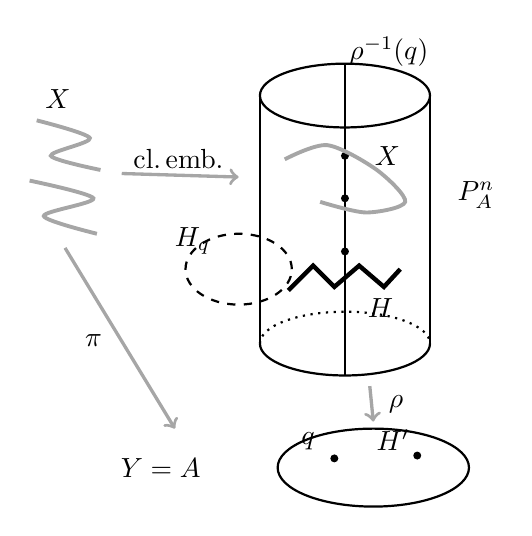
\begin{tikzpicture}[scale=0.9,line width=0.8pt]
  \draw (0,0.5) ellipse (1.2 and 0.45);
  \draw (-1.2,0.5) -- (-1.2,-3);
  \draw (1.2,0.5) -- (1.2,-3);
  \draw[dotted] (-1.2,-3) arc (180:0:1.2 and 0.45);
  \draw (-1.2,-3) arc (180:360:1.2 and 0.45);
  \node at (1.85,-0.9) {$\mathbb{P}^n_A$};
  \draw[thick] (0,0.95) -- (0,-3.45);
  \node at (0.62,1.12) {$\rho^{-1}(q)$};
  \fill (0,-0.35) circle (1.6pt);
  \fill (0,-0.95) circle (1.6pt);
  \fill (0,-1.7) circle (1.6pt);
  \draw[gray!70,line width=1.4pt] plot[smooth] coordinates {(-0.85,-0.4) (-0.25,-0.2) (0.45,-0.55) (0.85,-1.0) (0.3,-1.15) (-0.35,-1.0)};
  \node at (0.6,-0.35) {$X$};
  \draw[line width=1.6pt] (-0.8,-2.25) -- (-0.45,-1.9) -- (-0.15,-2.2) -- (0.2,-1.9) -- (0.55,-2.2) -- (0.78,-1.95);
  \node at (0.5,-2.5) {$H$};
  \draw[dashed] (-1.5,-1.95) ellipse (0.75 and 0.5);
  \node at (-2.15,-1.55) {$H_q$};
  \draw[gray!70,line width=1.4pt] plot[smooth] coordinates {(-4.35,0.15) (-3.6,-0.1) (-4.15,-0.35) (-3.45,-0.55)};
  \draw[gray!70,line width=1.4pt] plot[smooth] coordinates {(-4.45,-0.7) (-3.55,-0.95) (-4.25,-1.2) (-3.5,-1.45)};
  \node at (-4.05,0.45) {$X$};
  \draw[gray!70,line width=1.2pt,->] (-3.15,-0.6) -- (-1.5,-0.65);
  \node at (-2.35,-0.4) {$\mathrm{cl.\,emb.}$};
  \draw[gray!70,line width=1.2pt,->] (-3.95,-1.65) -- (-2.4,-4.2);
  \node at (-3.55,-2.95) {$\pi$};
  \draw (0.4,-4.75) ellipse (1.35 and 0.55);
  \fill (-0.15,-4.62) circle (1.6pt);
  \node at (-0.52,-4.38) {$q$};
  \fill (1.02,-4.58) circle (1.6pt);
  \node at (0.68,-4.36) {$H'$};
  \node at (-2.6,-4.75) {$Y=\Spec A$};
  \draw[gray!70,line width=1.2pt,->] (0.35,-3.6) -- (0.4,-4.1);
  \node at (0.72,-3.85) {$\rho$};
\end{tikzpicture}
\caption{\mbox{定理~18.1.6} 证明中的关键构造。（依原书手绘图重绘。）}\label{fig:finite-fibers-key-construction}
\end{figure}

\textbf{18.1.B.（练习：靶上纤维维数的\trUpperSemicontinuous{}性，就射影态射而言）}\quad 用与\mbox{定理~18.1.6} 中类似的手法，证明\emph{射影态射之纤维维数的\trUpperSemicontinuous{}性}（upper semicontinuity of fiber dimension of projective morphisms）：设 $\pi\colon X\to Y$ 是一个\trProjective\trMorphism，其中 $Y$ \trLocally\trNoetherian（或者更一般地，$\OO_Y$ 在自身上凝聚）。证明：$\{q\in Y\,:\,\dim\pi^{-1}(q)>k\}$ 是 $Y$ 的一个\trZariski\trClosedSubset。换言之，纤维的维数在靶的诸\trZariski\trClosedSubset{}上「跳跃」。（你可以把 $k=-1$ 的情形解读为「\trProjective\trMorphism{}都是闭的」这一事实——它基本上就是消元理论基本定理~8.4.10；参看 \S17.3.2。）这个练习对于体会\trProjective\trMorphism{}的行为方式而言相当重要。（\trVariety{}的情形早已在\mbox{定理~12.4.3(b)} 中做过；这条思路要简单得多。）

本节的最后一个练习则属另一个主题。

\textbf{18.1.C.（练习）}\quad 设 $0\to\mathscr{F}\to\mathscr{G}\to\mathscr{H}\to 0$ 是 $X$ 上诸\trQCSheaf{}的一个\trExactSequence，其中 $X$ 在 $A$ 上射影，而 $\mathscr{F}$ 凝聚。证明：当 $n\gg 0$ 时，
\[
0\longrightarrow \mathrm{H}^0(X,\mathscr{F}(n))\longrightarrow \mathrm{H}^0(X,\mathscr{G}(n))\longrightarrow \mathrm{H}^0(X,\mathscr{H}(n))\longrightarrow 0
\]
也正合。（提示：当 $n\gg 0$ 时，$\mathrm{H}^1(X,\mathscr{F}(n))=0$。）
